\documentclass[handout, notes=hide]{beamer}

\usepackage{attrib}
\graphicspath{{./figures/}}
\DeclareGraphicsExtensions{.pdf,.jpeg,.png,.jpg}
\usepackage[export]{adjustbox}

\usetheme{Rochester}
\usecolortheme{beaver}

\setbeamertemplate{bibliography entry title}{}
\setbeamertemplate{bibliography entry location}{}
\setbeamertemplate{bibliography entry note}{}

\renewcommand{\thefootnote}{\fnsymbol{footnote}}
\newcommand{\prescite}[1]{\footnote{\cite{#1}}}
\newcommand{\prestext}[1]{\footnotetext{\cite{#1}}}
\usepackage{perpage}
\MakePerPage{footnote}

\begin{document}

\title{The Quest to Replace Passwords}
\subtitle{R209, Paper by Joseph Bonneau, Cormac Herley, Paul C. van Oorschot, Frank Stajano, 2012}
\author{David Llewellyn-Jones}
\institute{
\href{mailto:David.Llewellyn-Jones@cl.cam.ac.uk}{David.Llewellyn-Jones@cl.cam.ac.uk}\\
Computer Laboratory\\
University of Cambridge}
\date{16th November 2015}

%%%%%%%%%%%%%%%%%%%%%%%%%%%%%%%%%%%%%%%%%

\frame{\titlepage}
\note{
Full title:

The Quest to Replace Passwords: A Framework for Comparative Evaluation of Web Authentication Schemes
}

%%%%%%%%%%%%%%%%%%%%%%%%%%%%%%%%%%%%%%%%%

\begin{frame}
\frametitle{The Quest to Replace Passwords}
\framesubtitle{A Framework for Comparative Evaluation of Web Authentication Schemes}
\setlength{\parskip}{0.5em}

Evaluation of Web password alternatives.

Compares 35 schemes against 25 properties.

Nine schemes in detail with the remaining 26 in the companion technical report.

\end{frame}
\note{
}

%%%%%%%%%%%%%%%%%%%%%%%%%%%%%%%%%%%%%%%%%

\begin{frame}
\frametitle{Pico}
\framesubtitle{No More Passwords!}

\begin{columns}[T]
\begin{column}[T]{0.6\textwidth}
\setlength{\parskip}{0.5em}

Core idea developed from Stajano's 2011 paper, grew from earlier work\footnotemark.

Emphasised failures of text-based passwords.

Summarised desirable properties of replacements systems.

Defined an `ideal' hardware-token-based approach (Pico).

Compared Pico against passwords.

\end{column}
\begin{column}[T]{0.4\textwidth}
\hspace{-1.5em}
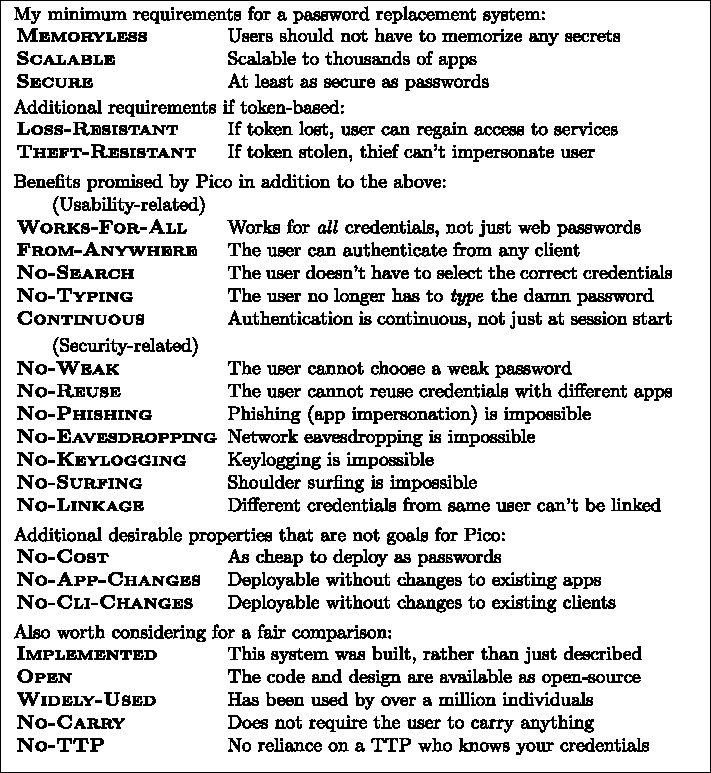
\includegraphics[width=1.1\textwidth]{stajano-properties}
\hspace{1.5em}
\end{column}
\end{columns}
\prestext{Stajano_2011, Stajano_2000}

\end{frame}
\note{
Frank Stajano, (2011). ``Pico: No More Passwords!''.

Frank Stajano, (2000). ``The Resurrecting Duckling -- What Next?''

Considering more than just Web.
}

%%%%%%%%%%%%%%%%%%%%%%%%%%%%%%%%%%%%%%%%%

\begin{frame}
\frametitle{Other Authors}
\framesubtitle{Domain Experts}
\setlength{\parskip}{0.5em}

\begin{enumerate}
\item {\bf Bonneau}: Completing PhD, mathematical framework for modelling human password choices\prescite{Bonneau_2012_phd}.
\item {\bf Herley}: Empirical investigation into password use\prescite{Florencio_2007}.
\item {\bf van Oorschot}: Development and evaluation of password alternative, graphical passwords\prescite{Chiasson_2012}.
\end{enumerate}

\centering 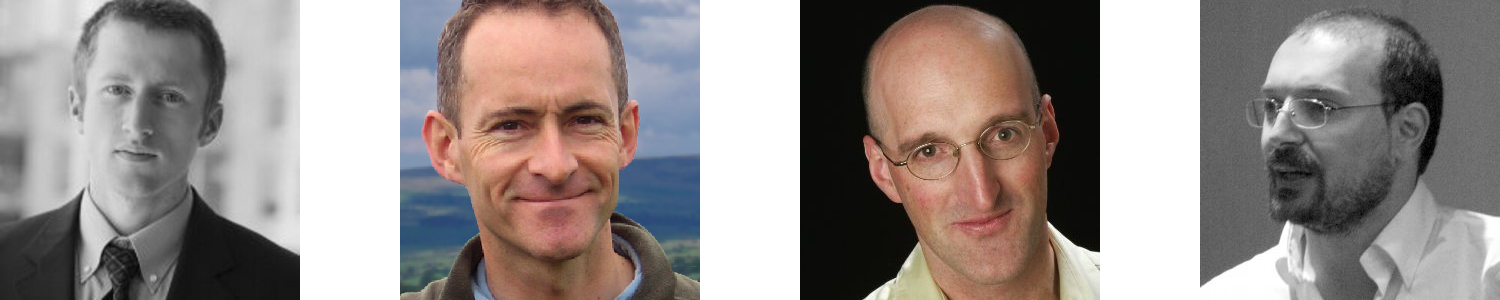
\includegraphics[width=0.7\textwidth]{authors-hor}

\end{frame}
\note{
\begin{enumerate}
\item Joseph Bonneau, University of Cambridge.
\item Cormac Herley, Microsoft Research.
\item Paul C. van Oorschot, Carleton University.
\item Frank Stajano, University of Cambridge.
\end{enumerate}

They each have different experiences both in terms of background in security, but also in methodological approaches.
}

%%%%%%%%%%%%%%%%%%%%%%%%%%%%%%%%%%%%%%%%%

\begin{frame}
\frametitle{Tragedy of the Commons}
\framesubtitle{}
\setlength{\parskip}{0.5em}

Bonneau had previously recognised password security as a {\it tragedy of the commons}.

\begin{quote}
Consumers' finite mental storage capacity for passwords is a common good from the viewpoint of website operators... Yet, each additional password places further demands on a user's memory, and may not bring real benefits to the user.
\attrib{Bonneau and Preibusch, 2010\/\prescite{Bonneau_2010}}
\end{quote}

\end{frame}
\note{
{\it Tragedy of the Commons}: a common good that has no financial barrier to use is depleted. Individuals each acting rationally act contrary to the benefit of the group.
}

%%%%%%%%%%%%%%%%%%%%%%%%%%%%%%%%%%%%%%%%%

\begin{frame}
\frametitle{Contributions}

The paper aims to provide more than just a comparative evaluation of schemes.
\begin{enumerate}
\item Comparison of password alternatives.
\item Provide a framework for comparative evaluation.
\item Understand how to develop successful alternatives.
\end{enumerate}

\end{frame}
\note{The framework is also described as a {\it methodology}.}

%%%%%%%%%%%%%%%%%%%%%%%%%%%%%%%%%%%%%%%%%

\begin{frame}
\frametitle{Heuristic Evaluation}
\setlength{\parskip}{0.5em}

\begin{columns}[T]
\begin{column}[T]{0.7\textwidth}
Broadly based on {\it Heuristic Evaluation} from usability engineering.
\begin{quotation}
[h]aving a small set of evaluators examine the interface and judge its compliance with recognized usability principles... Only after all evaluations have been completed are the evaluators allowed to communicate.
\attrib{Nielsen, 1994\/\footnotemark}
\end{quotation}
\end{column}
\begin{column}[T]{0.3\textwidth}
\hspace{-1.0cm}
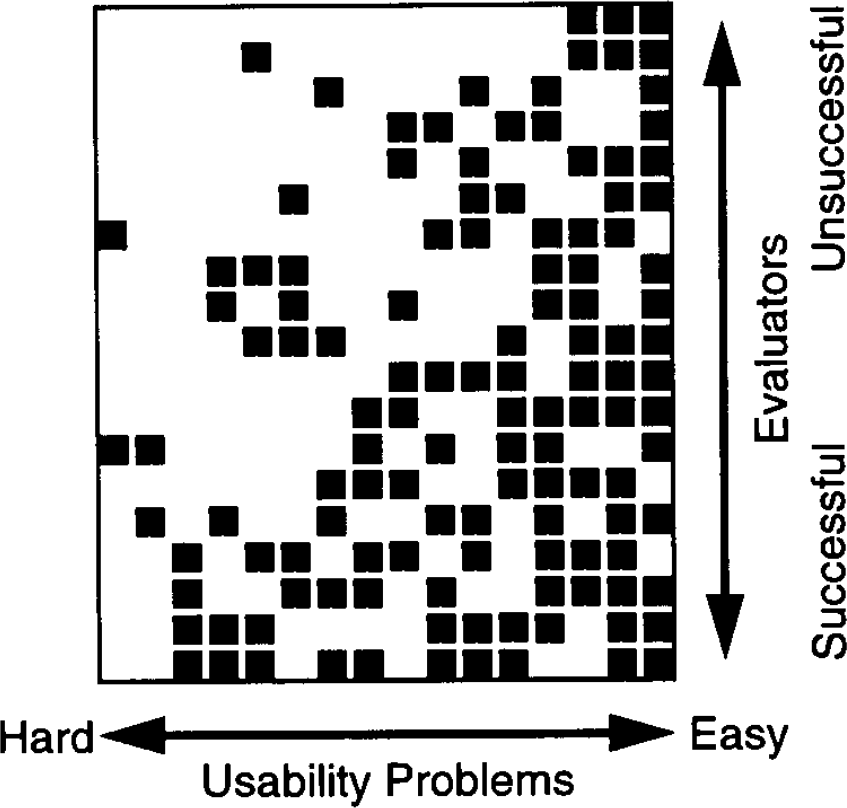
\includegraphics[width=1.3\textwidth,left]{heuristiceval}
\end{column}
\end{columns}
\prestext{Nielsen_1994}
\end{frame}
\note{
Nielson identified that experts identified different usability issues.

The optimum was between 3--5 experts, based on a cost-benefit analysis.

Nielsen, J. (1994). Heuristic Evaluation, page 2562. John Wiley \& Sons, Inc.

Discount usability engineering.
}

%%%%%%%%%%%%%%%%%%%%%%%%%%%%%%%%%%%%%%%%%

\begin{frame}
\frametitle{Methodology}
\setlength{\parskip}{0.5em}

\begin{enumerate}
\item Identify desirable characteristics, including single default comparator.
\item Have one expert evaluate the scheme against these characteristics.
\begin{enumerate}
\item Measured as either present, quasi or not present.
\item Determine whether better or worse than default.
\end{enumerate}
\item Other experts review assessment, challenge and discuss if disagreement.
\item Other experts cross-validate results.
\end{enumerate}

\end{frame}
\note{
Evaluating security is a particularly challenging task.

The approach can be contrasted with {\it empirical quantitative\/} approaches and {\it analytical approaches}.
}

%%%%%%%%%%%%%%%%%%%%%%%%%%%%%%%%%%%%%%%%%

\begin{frame}
\frametitle{Usability -- Deployability -- Security}
\framesubtitle{}
\setlength{\parskip}{0.5em}

Starts from a positive position of identifying alternatives, generates a deeper understanding of why alternatives have failed.

Exposed through a broadening of the evaluation criteria, {\it UDS evaluation framework}:
\begin{enumerate}
\item Usability.
\item Deployability.
\item Security.
\end{enumerate}

\end{frame}
\note{
}

%%%%%%%%%%%%%%%%%%%%%%%%%%%%%%%%%%%%%%%%%

\begin{frame}
\frametitle{Desirable properties}
\framesubtitle{}
\setlength{\parskip}{0.5em}
\scriptsize
\begin{tabular}{l l}
{\bf Usability benefits} & \\
U1 - Memorywise-Effortless & U2 - Scalable-for-Users \\
U3 - Nothing-to-Carry & U4 - Physically-Effortless \\
U5 - Easy-to-Learn & U6 - Efficient-to-Use \\
U7 - Infrequent Errors & U8 - Easy-Recovery-from-Loss \\
& \\
{\bf Deployability benefits} & \\
D1 - Accessible & D2 - Negligible-Cost-per-User \\
D3 - Server-Compatible & D4 - Browser-Compatible \\
D5 - Mature & D6 - Non-Proprietary \\
& \\
{\bf Security benefits} & \\
S1 - Resilient-to-Physical-Observation & S2 - Resilient-to-Targeted-Impersonation  \\
S3 - Resilient-to-Throttled-Guessing & S4 - Resilient-to-Unthrottled-Guessing \\
S5 - Resilient-to-Internal-Observation & S6 - Resilient-to-Leaks-from-Other-Verifiers \\
S7 - Resilient-to-Phishing & S8 - Resilient-to-Theft \\
S9 - No-Trusted-Third-Party & S10 - Require-Explicit-Consent \\
S11 - Unlinkable & \\
\end{tabular}
\end{frame}
\note{
Consider:
\begin{enumerate}
\item U1 - Memorywise-Effortless
\item D3 - Server-Compatible
\item S11 - Unlinkable
\end{enumerate}

Table of results on page 11.
}

%%%%%%%%%%%%%%%%%%%%%%%%%%%%%%%%%%%%%%%%%

\begin{frame}
\frametitle{}
\framesubtitle{}
\setlength{\parskip}{0.5em}

Interesting points about the approach:
\begin{enumerate}
\item Explicitly haven't provided totals.
\item Properties cold be weighted depending on scenario.
\item Considered having `fatal' and `power-user' ratings.
\item Some characteristics mutually incompatible.
\item Prefer `broadly right' to `precisely wrong'.
\item Aim to avoid evaluator bias.
\end{enumerate}

\end{frame}
\note{
Lack of totals seen previously in the Anderson et al. paper ``Measuring the Cost of Cybercrime''\prescite{Anderson_2013}.

Bias: Contrasts with Heuristic Evaluation, aiming at problem identification rather than comparative evaluation. Problem identification can be likened to code review.

Use of several experts intended to reduce risk of bias.
Can consider the Pico results:
\begin{enumerate}
\item {\bf Sixteen} equivalent properties, {\bf six} only considered in Pico paper, {\bf nine} additional for the framework.
\item Differences:
\begin{enumerate}
\item U8 - Easy-recovery-from-loss (dropped).
\item S8 - Resilient-to-theft (reduced to Quasi).
\end{enumerate}
\end{enumerate}

Incompatible: Memorwise-Effortless (U1), Nothing-to-Carry (U3).
}
%%%%%%%%%%%%%%%%%%%%%%%%%%%%%%%%%%%%%%%%%

\begin{frame}
\frametitle{The Results}
\framesubtitle{}
\setlength{\parskip}{0.5em}

The authors emphasise {\it the journey}.
\begin{quotation}
``the journey (the rating exercise) is the reward''
\end{quotation}
Also more tangible outcomes about password replacements.
\begin{enumerate}
\item ``most schemes do better than passwords on security''
\item ``some schemes do better and some do worse on usability''
\item ``every scheme does worse than passwords on deployability''
\end{enumerate}
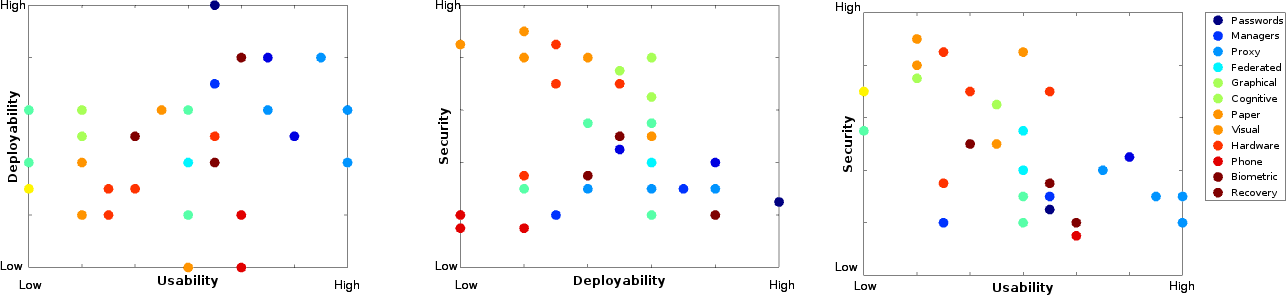
\includegraphics[width=1.0\textwidth]{summaryflat}

\end{frame}
\note{
``the important technical insights we gained about schemes by discussing whether our ratings were fair and consistent were worth much more to us than the actual scores produced. As a take-home message for the value of this exercise, bringing a team of experts to a shared understanding of the relevant technical issues is much more valuable than ranking the schemes linearly or reaching unanimous agreement over scoring.''
\begin{enumerate}
\item Security: given this is the most common aim, not surprising.
\item Usability: Federated/Single-Sign-On approaches do well.
\item Usability: Biometrics do well, but fail on security properties.
\item Deployability: Everything does poorly; not surprising. Password managers do the best.
\end{enumerate}
Overall, Federated passwords appear most promising.
}

%%%%%%%%%%%%%%%%%%%%%%%%%%%%%%%%%%%%%%%%%

\begin{frame}
\frametitle{Methodology Reuse}
\framesubtitle{Strengthening User Authentication through Opportunistic Cryptographic Identity Assertions}
\setlength{\parskip}{0.5em}

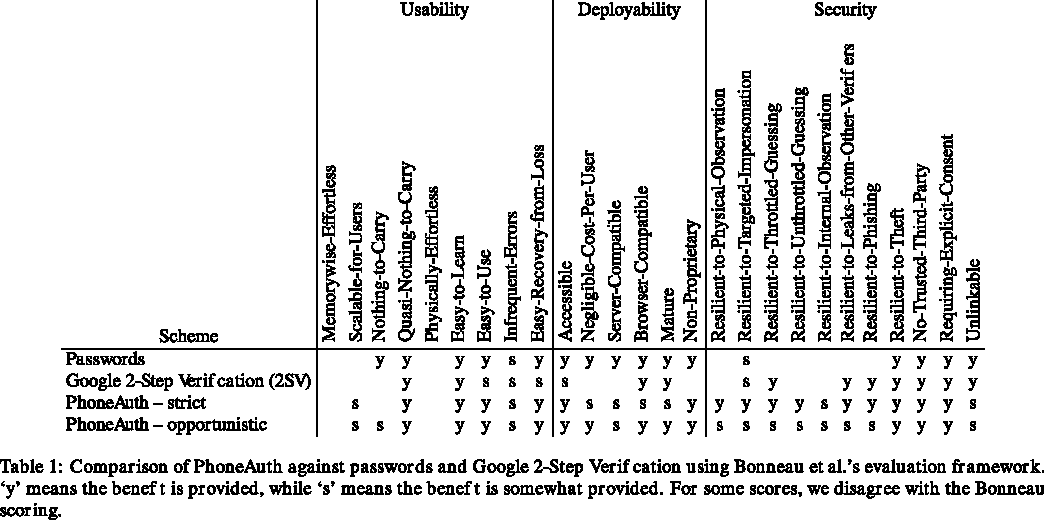
\includegraphics[width=\textwidth]{czeskis2012}
\prescite{Czeskis_2012}

\end{frame}
\note{
Czeskis, A., Dietz, M., Kohno, T., Wallach, D., and Balfanz, D. (2012). ``Strengthening User Authentication Through Opportunistic Cryptographic Identity Assertions''.

PhoneAuth, authenticates using phone and opportunistically providing cryptographic identity assertions.
}

%%%%%%%%%%%%%%%%%%%%%%%%%%%%%%%%%%%%%%%%%

\begin{frame}
\frametitle{Methodology Reuse}
\framesubtitle{
Designing Leakage-resilient Password Entry on Touchscreen Mobile Devices\\
{ZEBRA}: Zero-Effort Bilateral Recurring Authentication}
\setlength{\parskip}{0.5em}

\begin{columns}[T]
\begin{column}[c]{0.5\textwidth}
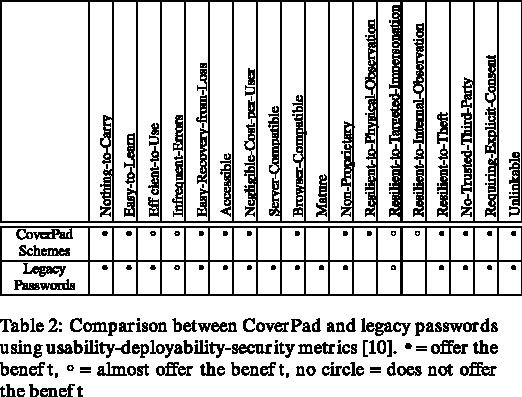
\includegraphics[width=1.0\textwidth]{yan2013}
\end{column}
\begin{column}[c]{0.5\textwidth}
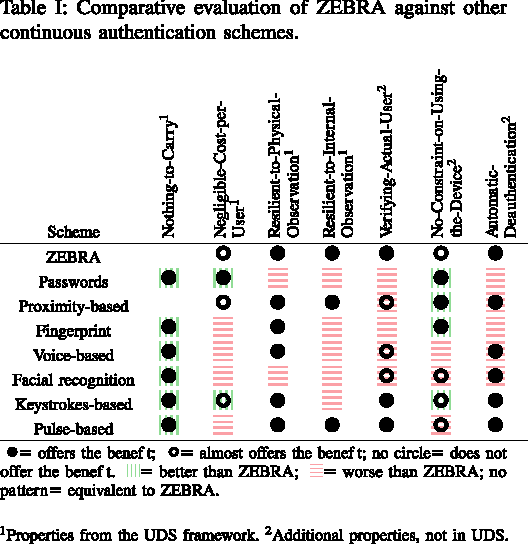
\includegraphics[width=1.0\textwidth]{mare2014}
\end{column}
\end{columns}
\prestext{Yan_2013, Mare_2014}

\end{frame}
\note{
Yan, Q., Han, J., Li, Y., Zhou, J., and Deng, R. H. (2013). ``Designing Leakage-resilient Password Entry on Touchscreen Mobile Devices''.

CoverPad touchscreen password entry.

Mare, S., Markham, A., Cornelius, C., Peterson, R., and Kotz, D. (2014). ''ZEBRA: Zero-Effort Bilateral Recurring Authentication''.

ZEBRA: Zero-Effort Bilateral Recurring Authentication. Correlates wrist movement with keyboard/mouse activity.
}

%%%%%%%%%%%%%%%%%%%%%%%%%%%%%%%%%%%%%%%%%

\begin{frame}
\frametitle{Conclusion}
\setlength{\parskip}{0.5em}

What starts out as a means of `discrediting' passwords results in a far more nuanced picture.

There is no perfect solution.

Deployability is crucial: passwords benefit from the commons.

The methodology offers a more realistic approach to understanding success of security mechanisms.

\end{frame}
\note{
}

%%%%%%%%%%%%%%%%%%%%%%%%%%%%%%%%%%%%%%%%%

\begin{frame}
\frametitle{Bibliography}
{\tiny
\bibliographystyle{apalike}
\bibliography{main}
}%
\end{frame}

%%%%%%%%%%%%%%%%%%%%%%%%%%%%%%%%%%%%%%%%%

\end{document}
